\chapter{Implementation}

%The implementation should discuss any issues you encountered as you tried to implement your design. During the work, you might have found that elements of your design were unnecessary or overly complex; perhaps third-party libraries were available that simplified some of the functions that you intended to implement. If things were easier in some areas, then how did you adapt your project to take account of your findings?
%
%It is more likely that things were more complex than you first thought. In particular, were there any problems or difficulties that you found during implementation that you had to address? Did such problems simply delay you or were they more significant?
%
%You can conclude this section by reviewing the end of the implementation stage against the planned requirements. 

\section{Code Implementation \& Third-Party libraries}
As seen below the Website and Discord bot have been split up into two separate sections because during implementation I decided to make the systems separate. This helps with code maintainability, readability and allows the administrator who sets up this project to deploy the website and bot services on different containers or networks. For more information of third party libraries please see appendix A.

\subsection{Website Building and Final Design}
To create and run the website I've used a set of different libraries to perform certain tasks. Firstly I've used the Apache2 \cite{apache2} web hosting framework to host the website along with the library libapache2-mod-auth-openidc to reroute all incoming traffic to OpenID Connect \cite{OpenID} for user authentication. On top of these I have used the linux tool certbot \cite{certbot} to create a Let's Encrypt certificate for the website to enable HTTPS. 

As discussed previously in this document in section \ref{sec1:Research} there were many libraries that were considered when deciding on the website framework. Django \cite{Django} was the framework of choice and it is open-source and free to use on personal projects. It is also very useful as it generates the majority of the code required to create and run a website so most of the code used will be picked up by the system for UAP. Apart from the general template I created a "Django Application" called login that contains the files and code which is used to run the website. I can confirm that the folder, login, is all my own code and shouldn't fall under UAP.

The website pages also use a third party library called bootstrap \cite{bootstrap} that is used to generate responsive mobile-first CSS for the website. The final design of the website ended up being very similar to that of the mockups I made in section \ref{sec2:ui} and included below are some images from the final website.

\textbf{Note}: The navigation bars in the images below are smaller than the mockups due to the change in screen size. These images were taken on a 27inch monitor whereas the mockups were made for a 15inch monitor.

\begin{figure}[H]
	\centering
	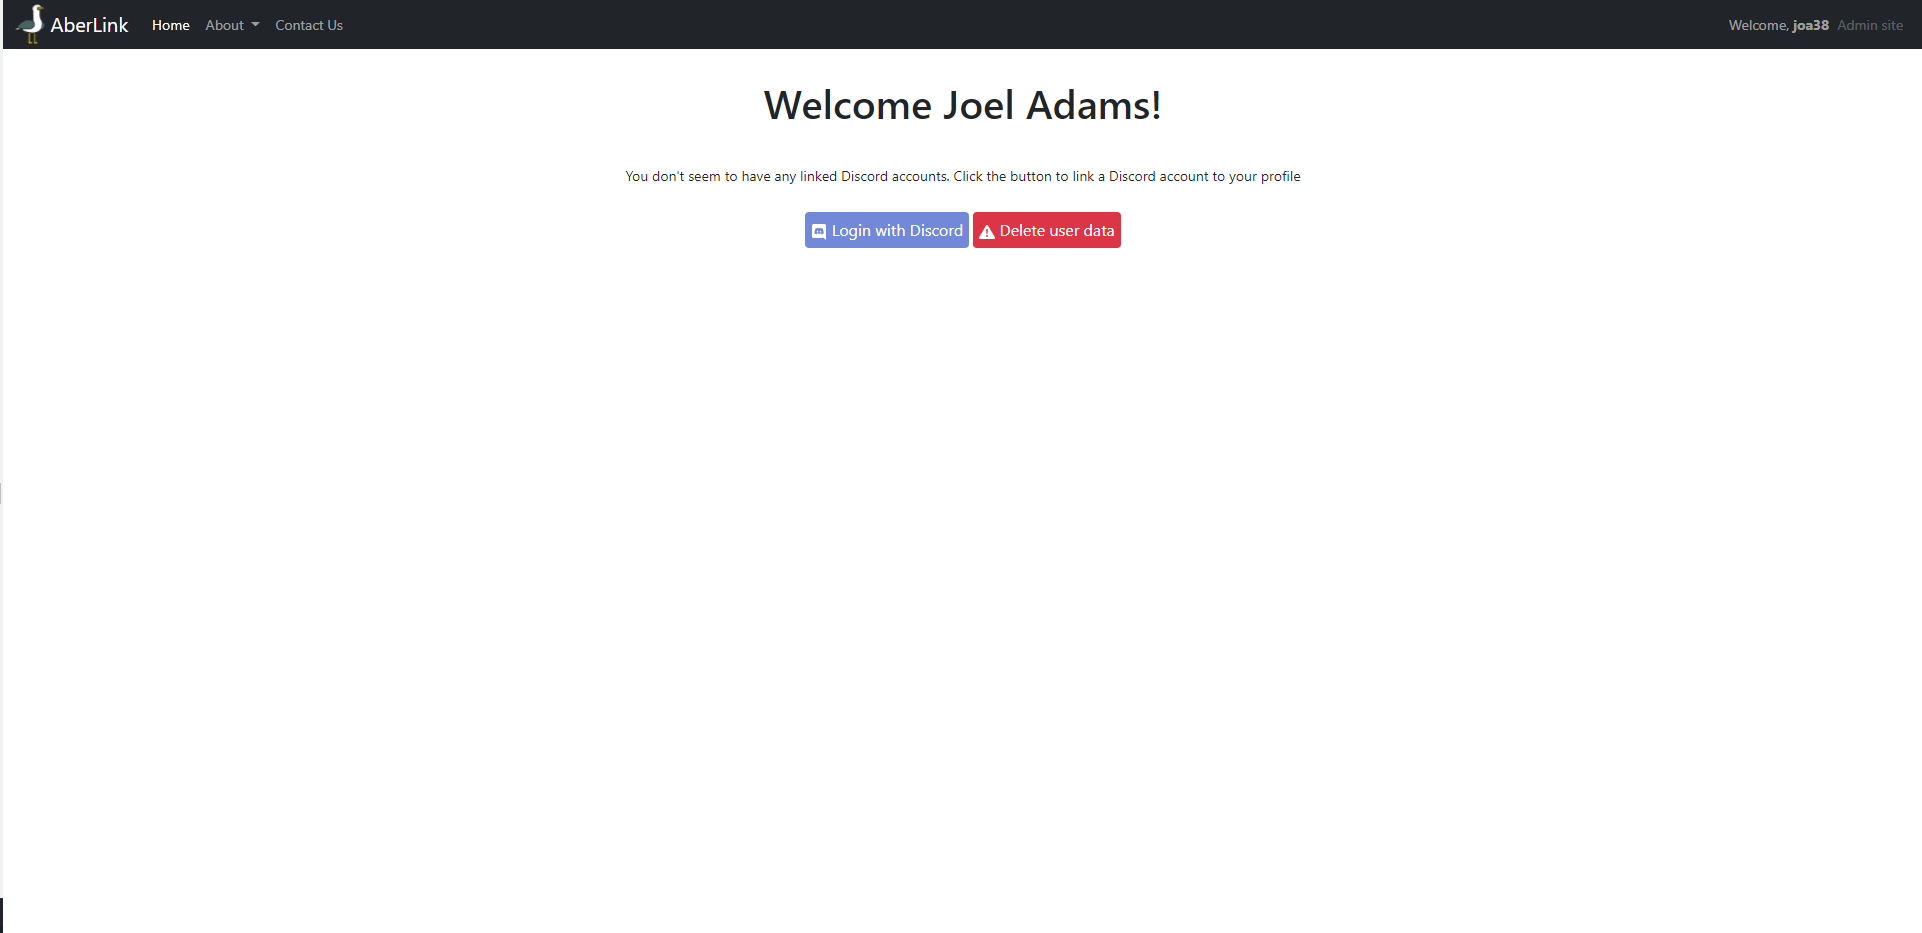
\includegraphics[width=1\linewidth]{Figures/website-acc-0.png}
	\caption{Final website with 0 linked Discord accounts}
	\label{fig:final-web-acc-0}
\end{figure}

\begin{figure}[H]
	\centering
	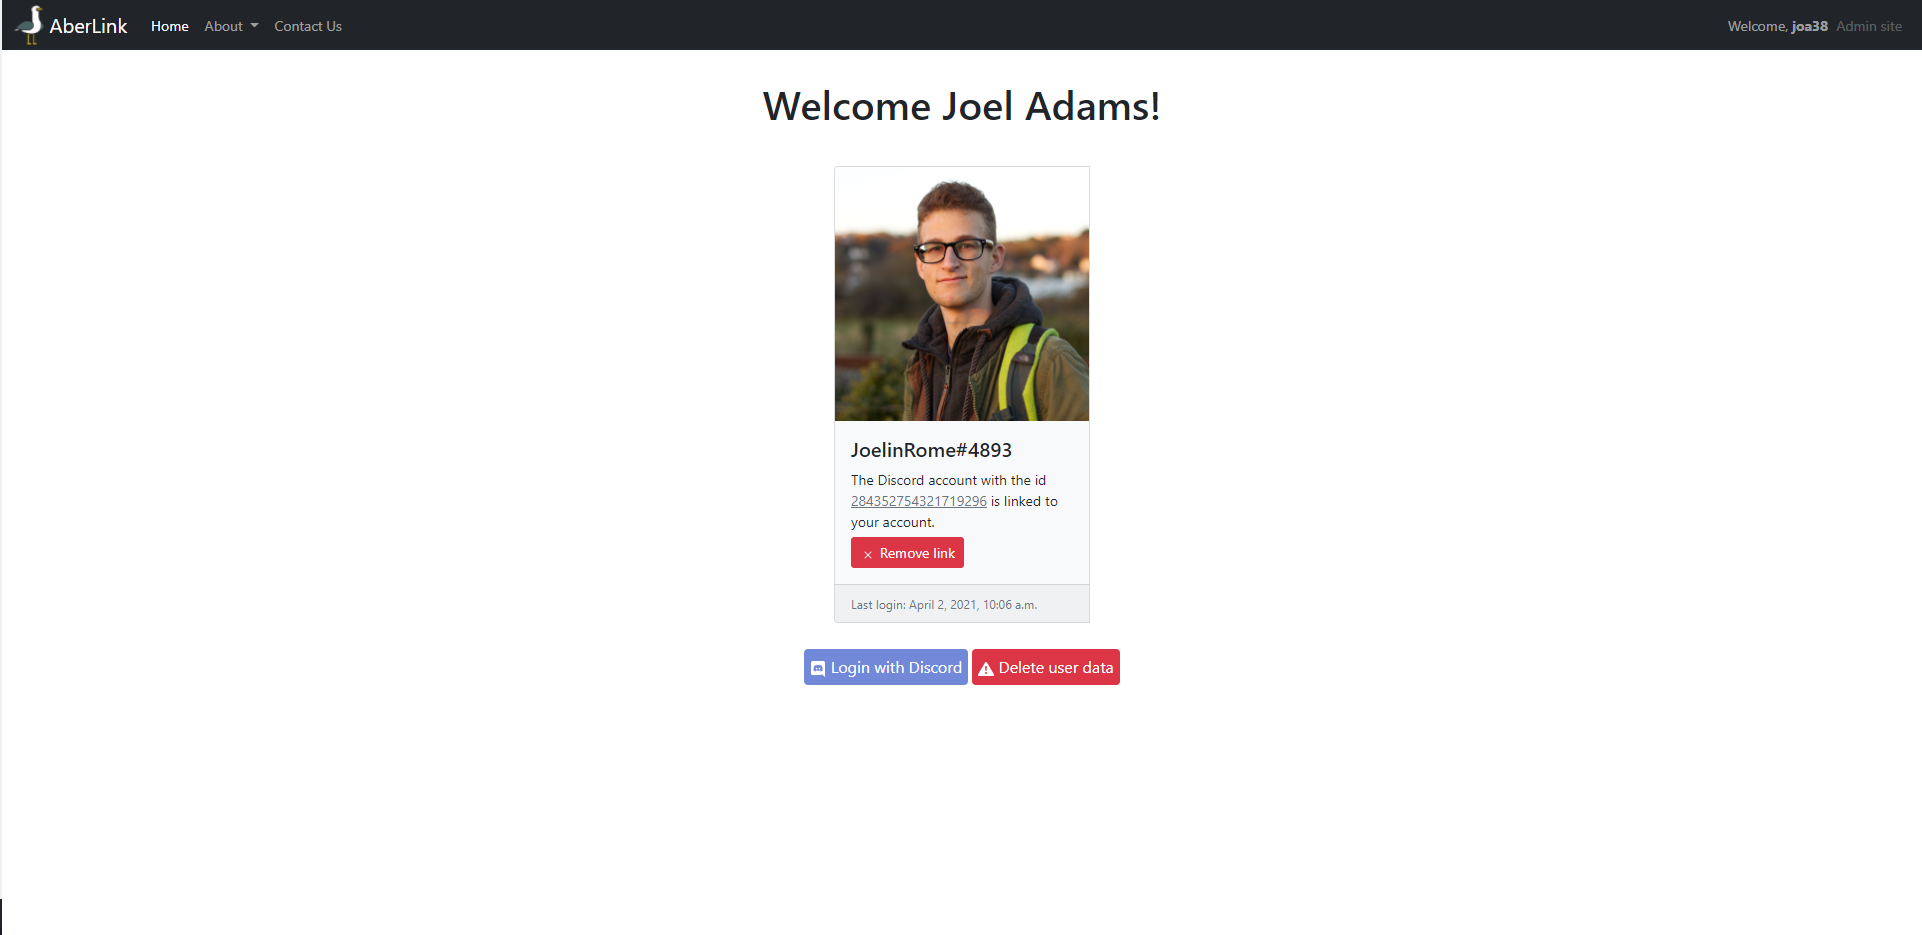
\includegraphics[width=1\linewidth]{Figures/website-acc-1.png}
	\caption{Final website with 1 linked Discord accounts}
	\label{fig:final-web-acc-1}
\end{figure}

\begin{figure}[H]
	\centering
	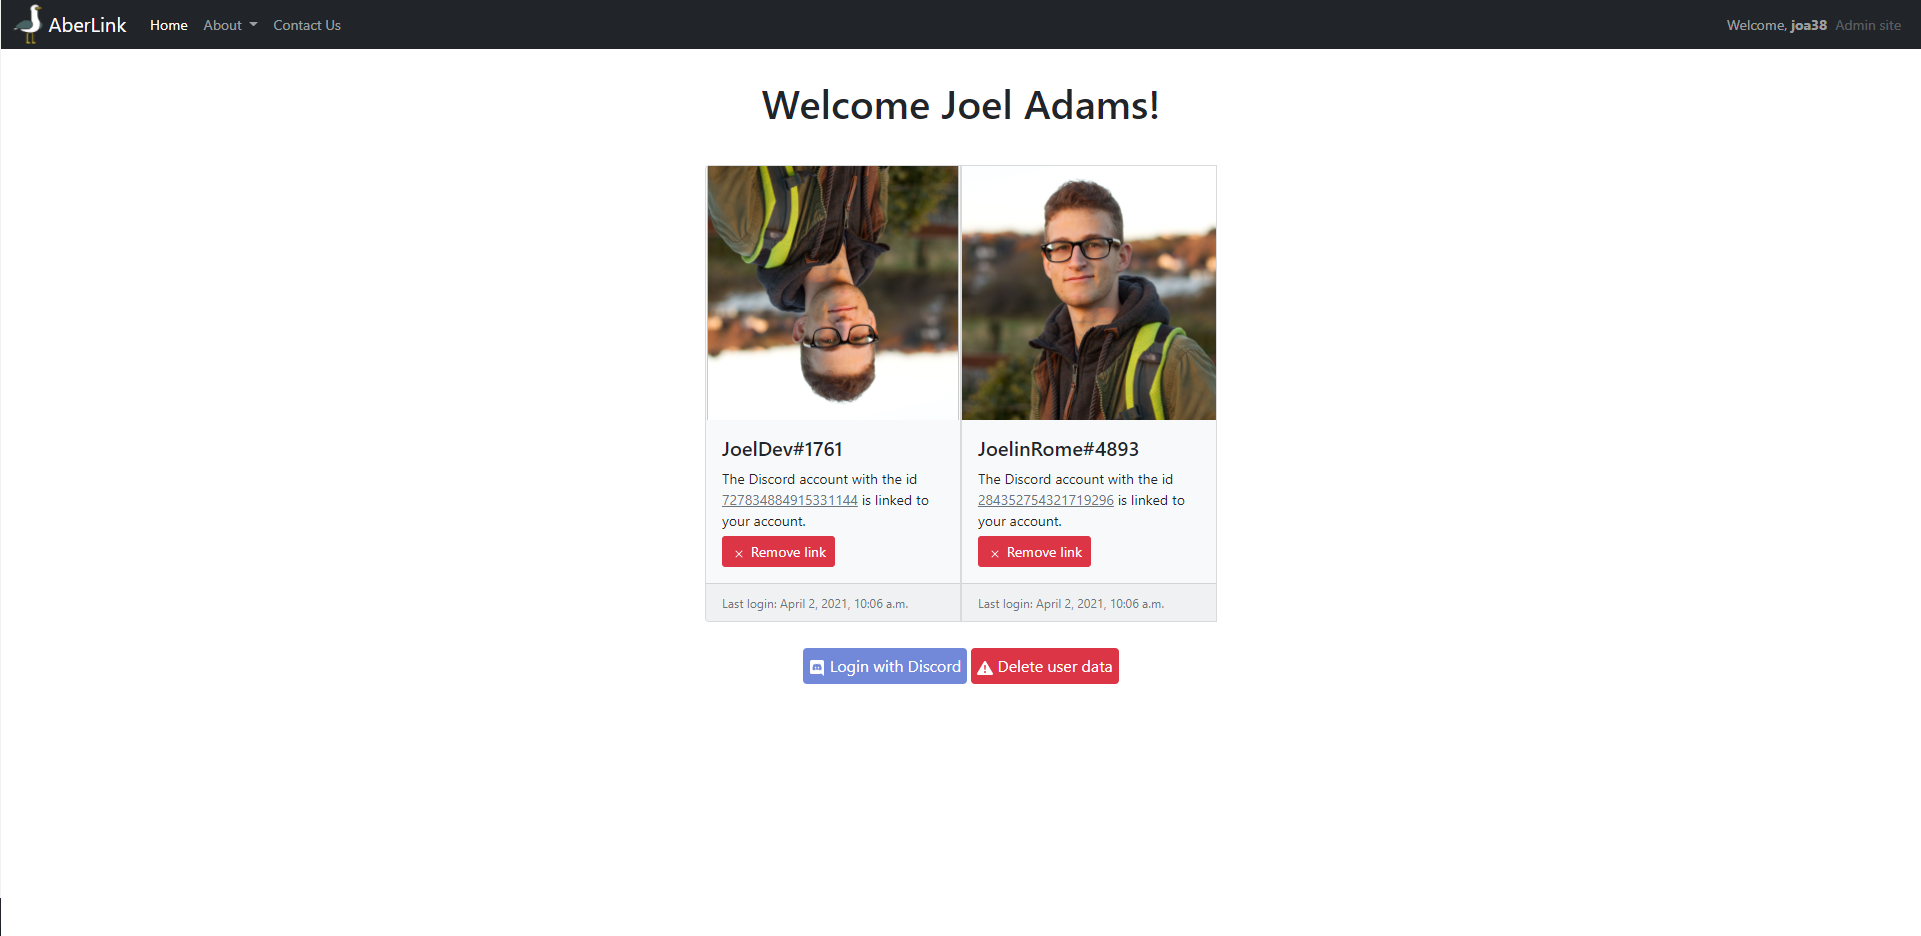
\includegraphics[width=1\linewidth]{Figures/website-acc-2.png}
	\caption{Final website with 2 linked Discord accounts}
	\label{fig:final-web-acc-2}
\end{figure}

\begin{figure}[H]
	\centering
	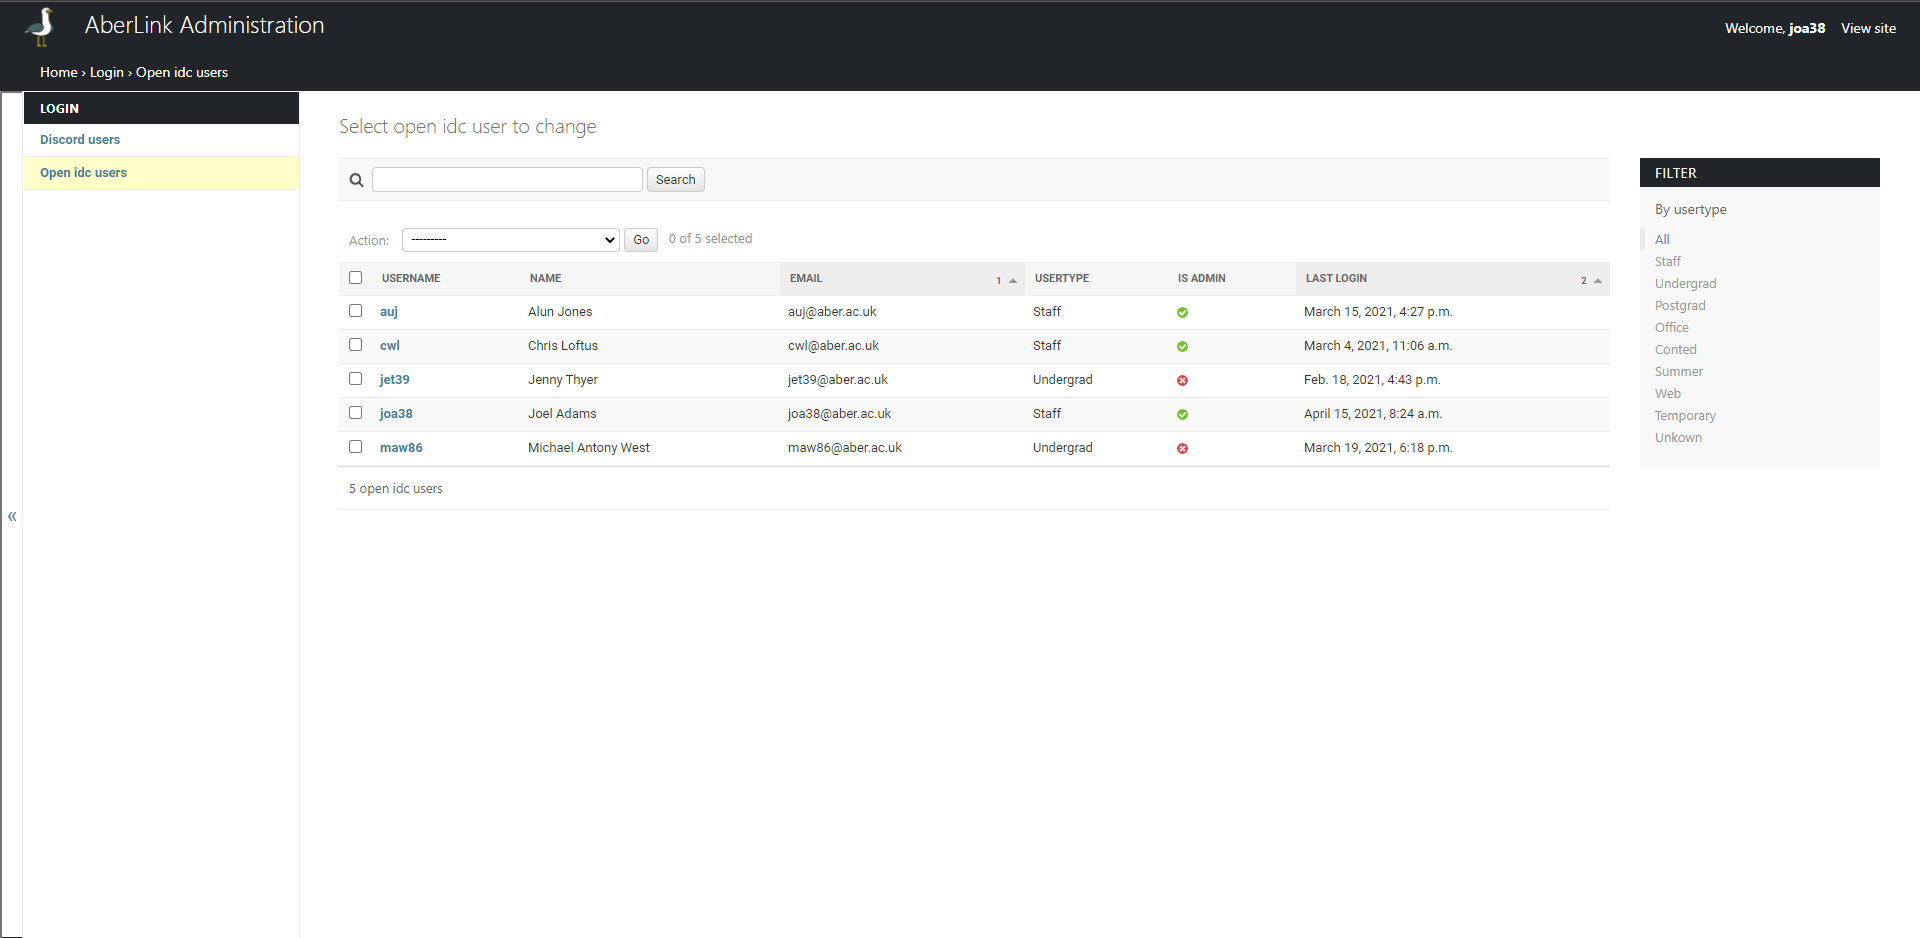
\includegraphics[width=1\linewidth]{Figures/website-admin-openidc.png}
	\caption{Final website Admin page for Aber accounts}
	\label{fig:final-web-admin-openidc}
\end{figure}

\begin{figure}[H]
	\centering
	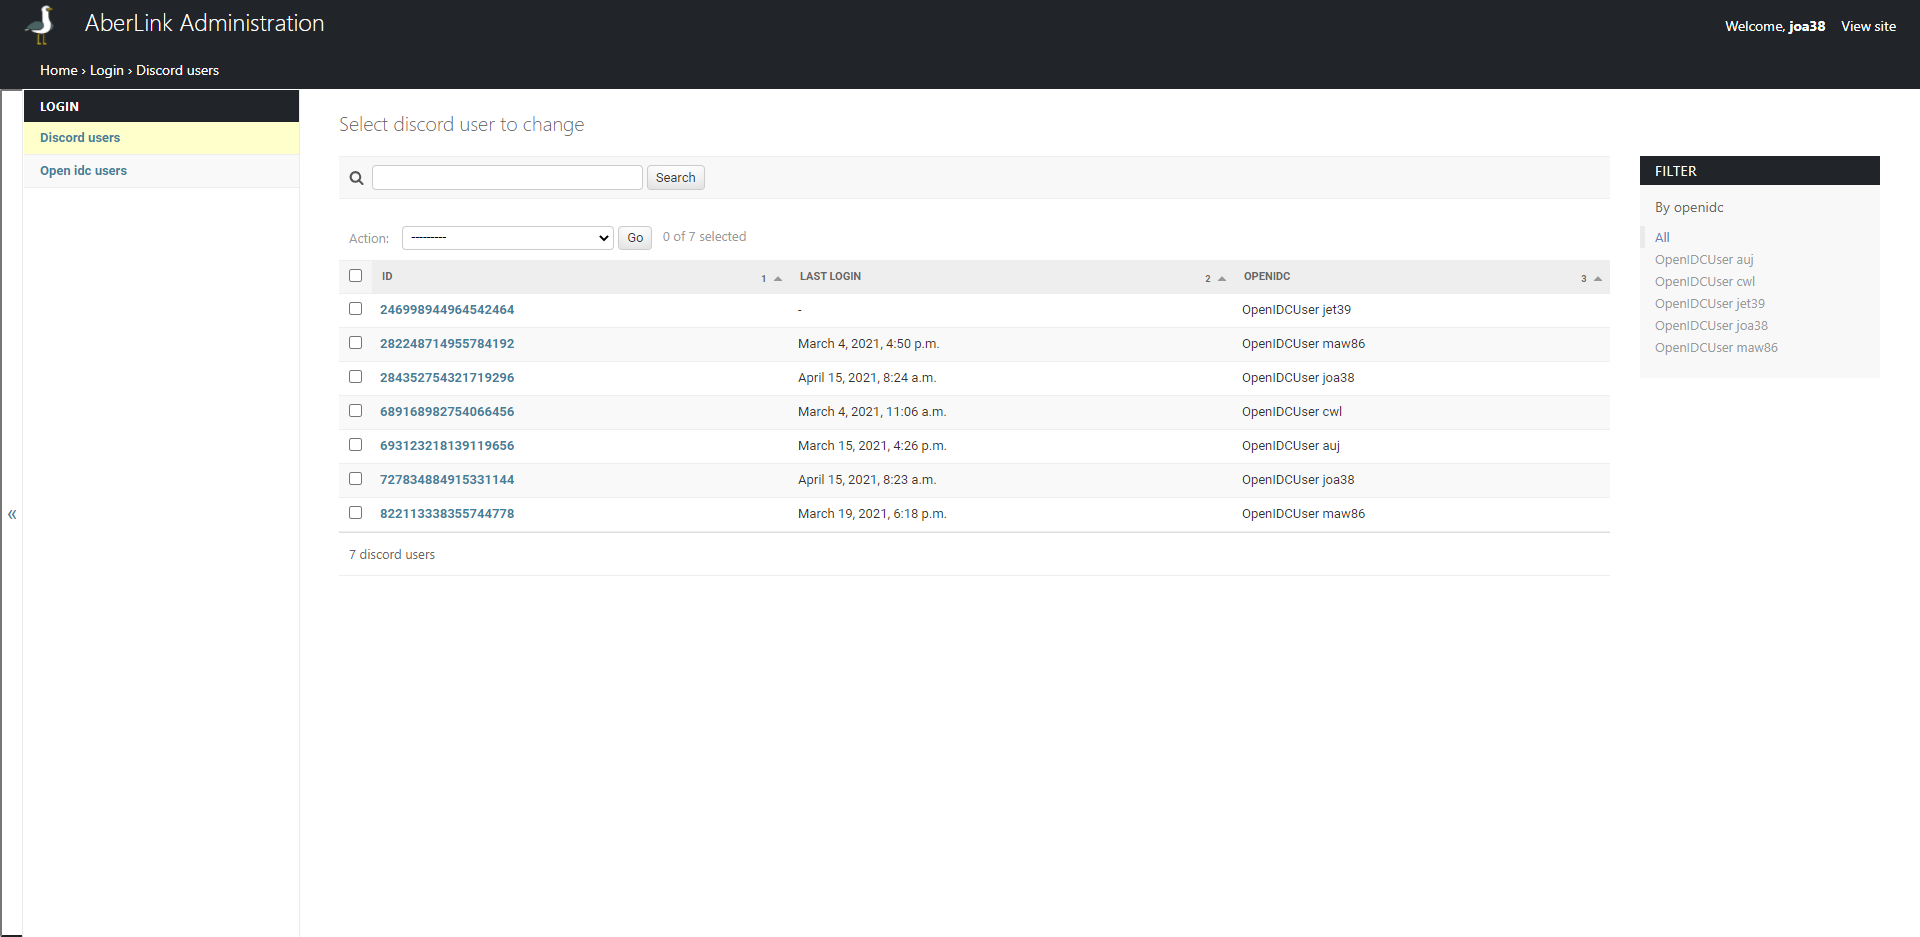
\includegraphics[width=1\linewidth]{Figures/website-admin-discord.png}
	\caption{Final website Admin page for Discord accounts}
	\label{fig:final-web-admin-dis}
\end{figure}

\subsection{Discord Bot}
The Discord bot (AberLink) implementation is exactly as described in the section \ref{sec2:discord} of the design. AberLink uses the Python library Discord.py \cite{discord.py} to make calls to and from the Discord API and to interact with the database it uses the Python library Psycopg2 \cite{psycopg2}. Both of these pieces of software are open-source and free to use in personal projects. 

\subsection{Database}
The Database implementation was relatively straight forward as Django \cite{Django} generates all of the required tables for the project to function once you define the models. I've included the model used to generate OpenID Connect \cite{OpenID} aber user model below. In this figure you can see that there are two classes; OpenIDCUserManager to create a new database object and OpenIDCUser to make the database model. 

The OpenIDCUserManager class has three main parameters; one to call itself, a user which is a JSON object and password which is defaulted to None as no password data is stored. The information from the user object is passed throughout the code and is used to decide if the user should have admin permissions. The user is then saved to the database.

The OpenIDCUser class contains a nested class called usertypes that is a list of all the possible choices for incoming usertypes from user authentication. Further down we can see that there is a set of definitions for the database model such as the id, username, name, etc. Note however that the usertype definition uses the choices class to define what role a user may have. As this model is the main model used to authenticate users on the website Django requires that the model contains a few special items including a password which I have set to None and the arrays at the bottom called USERNAME\_FIELD and REQUIRED\_FIELDS.

\begin{figure}[H]
\begin{lstlisting}[language=Python]
class OpenIDCUserManager(BaseUserManager):
    def create_user(self, user, password=None):
        new_user = self.model(
            username = user['OIDC_CLAIM_preferred_username'],
            name = user['OIDC_CLAIM_name'],
            email = user['OIDC_CLAIM_email'],
            usertype = user['OIDC_CLAIM_usertype']
        )
        if user['OIDC_CLAIM_usertype'] == "staff":
            new_user.is_admin = True
        new_user.save(using=self._db)
        return new_user

class OpenIDCUser(AbstractBaseUser):
    objects = OpenIDCUserManager()

    class usertypes(models.TextChoices):
        STAFF = 'staff'
        UNDERGRAD = 'undergrad'
        POSTGRAD = 'postgrad'
        OFFICE = 'office'
        CONTED = 'conted'
        SUMMER = 'summer'
        WEB = 'web'
        TEMPORARY = 'temporary'
        UNKNOWN = 'unknown'

    id = models.AutoField(auto_created=True, primary_key=True, serialize=False)
    username = models.CharField(max_length=40)
    name = models.CharField(max_length=300)
    email = models.CharField(max_length=30)
    usertype = models.CharField(max_length=50, choices=usertypes.choices)
    last_login = models.DateTimeField(null=True)
    password = None
    is_active = models.BooleanField(default=True)
    is_admin = models.BooleanField(default=False)

    USERNAME_FIELD = 'id'
    REQUIRED_FIELDS = ['username', 'name', 'email', 'usertype']
\end{lstlisting}
\caption{Django database model of OpenID Connect Aber users}
\label{fig:django-database}
\end{figure}

The tables generated for the database are pictured below and they do differ quite drastically from the tables discussed during the design section \ref{sec2:database}. This is because I was not originally accounting for the tables that get automatically generated by Django \cite{Django} that are required for the application to run. I have included information below the figure to explain what the tables mean.

\begin{figure}[H]
	\centering
	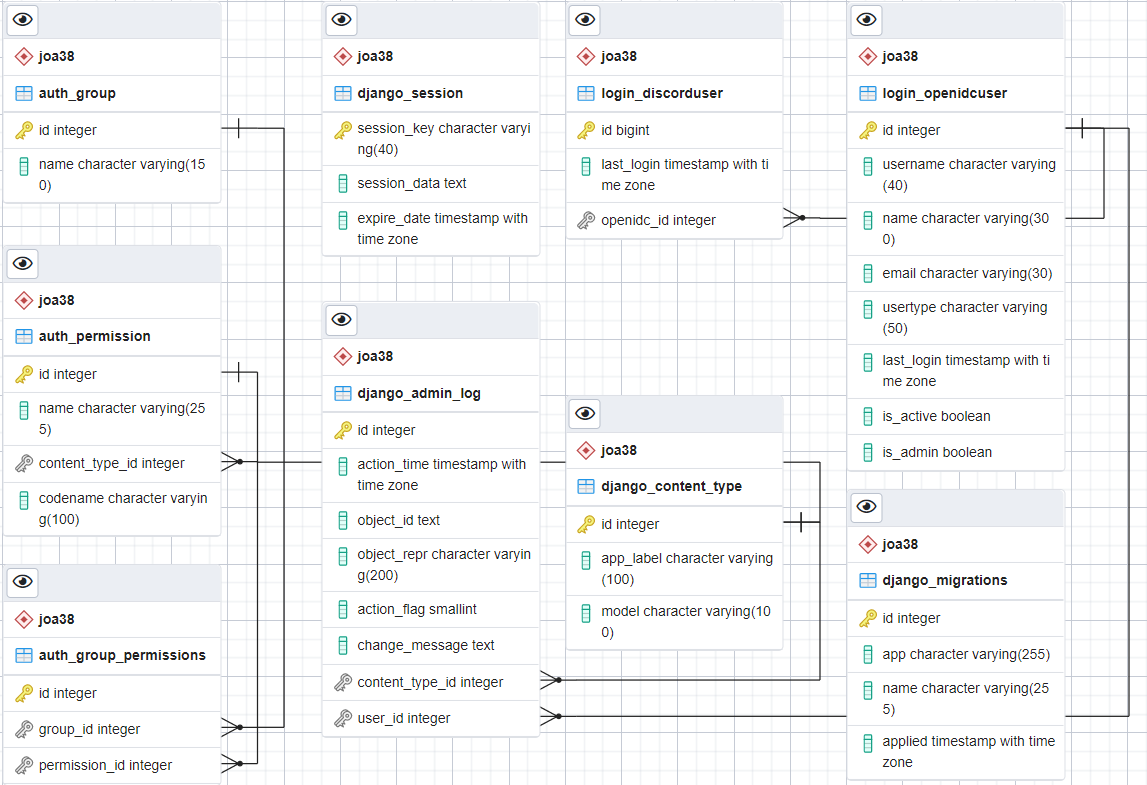
\includegraphics[width=1\linewidth]{Figures/er-diagram.png}
	\caption{Final Entity Relationship diagram for database}
	\label{fig:final-database}
\end{figure}

\begin{itemize}
	\item \textbf{User tables} - These two tables are the ones that have been discussed previously in this document for storing user data.
	\begin{itemize}
		\item \textbf{login\_openidcuser} - This table stores the OpenID Connect \cite{OpenID} information and is used as the authenticated user account.
		\item \textbf{login\_discorduser} - This table stores information on the discord user and contains a foreign key relationship with the table above.
	\end{itemize}
	\item \textbf{Django tables} - Tables generated by Django \cite{Django}
	\begin{itemize}
		\item \textbf{django\_migrations} - This table contains the history of the changes made to the database using Django. It acts as a way to revert to previous versions of the database in the case of 
		errors.
		\item \textbf{django\_session} - Stores sessions on the currently logged in users.
		\item \textbf{django\_content\_type} - Stores information on all available models in the database.
		\item \textbf{django\_admin\_log} - Stores history of logins for administrative users.
		\item \textbf{auth\_group \& auth\_group\_permissions \& auth\_permissions} - These tables are part of the backend for the authentication of users.
	\end{itemize}
\end{itemize}

\section{Unforeseen Issues}\label{sec3:unforeseen}
An issue that I encountered was with creating the custom user model in Django that would have been used to model the database. The documentation and videos I found online about implementing user models were rather cryptic and difficult to understand, however I eventually found a video explaining how to implement a good custom user model. Once this was completed I realised that Django isn't happy with modelling the primary key of a table using a char so I had to switch to using an int. This turned out to be a good idea as Aberystwyth university tends to recycle old emails so over the next 5 years there could be an issue where the database would try and create a new entry in the database with the same email.

\section{Review Against Planned Requirements}
Most of the planned requirements haven't changed during implementation however as discussed in the section above \ref{sec3:unforeseen} the database model has changed slightly and the updated diagram is included below.
\begin{figure}[H]
	\centering
	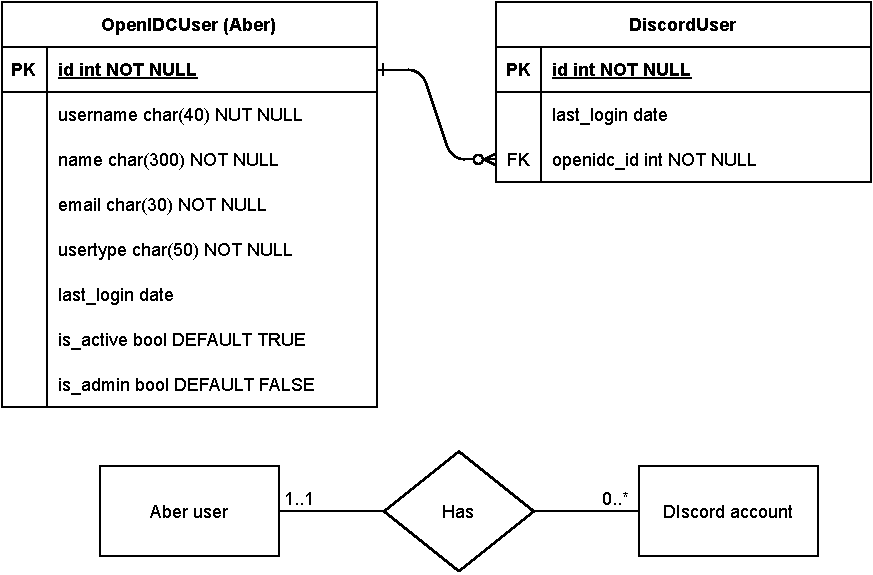
\includegraphics[width=0.8\linewidth]{Figures/database-er-1}
	\caption{Updated Entity relationship diagram for database}
	\label{fig:database-er-1}
\end{figure}

The planned requirements also included a section called \textbf{Interface for lecturers and students on website} has also only been partially fulfilled. I have completed the second part of this task which was to create admin pages to view the connected staff and students however the first part where users can view what servers they are in is missing. This was a design choice that I made because I realised that this would require that Discord servers are added to database and that they would have to be updated when any issues occurred. This was also bad because this list would have to be maintained and couldn't be automatically updated which would lead to it breaking down the line.

In the final section of the planned requirements \textbf{Further potential work} I have decided against integrating DemoHelper into AberLink as this would greatly increase it's complexity and make it much more difficult to maintain.